\section{Research plan}


\vspace{2mm}
\hrule
\textit{`Much of the variation in healthcare is accounted for by the willingness and ability of doctors to offer treatment rather than differences in illness or patient preference'} John Wennberg, the pioneer of research into clinical variation and founder of the Dartmouth Atlas of Health Care.
\vspace{2mm}
\hrule

\subsection{What is the problem?}


Stroke remains one of the leading causes of death and disability, globally and in the UK. The majority of strokes are caused by a clot. Clots may be reduced or removed with \textit{reperfusion} treatments if given soon enough after a stroke. These treatments include thrombolysis, a clot-busting medication given by injection/infusion \cite{emberson_effect_2014} and, more recently, thrombectomy, mechanical removal of a clot performed in a specialist centre \cite{fransen_time_2016}.

Despite thrombolysis being long-established and of proven benefit in ischaemic stroke, use of thrombolysis varies significantly both between and within European countries \cite{aguiar_de_sousa_access_2019}. In England and Wales the national stroke audit reported that in 2021/22, 20 years on from the original European Medicines Agency licensing of alteplase for acute ischaemic stroke, thrombolysis rates for emergency stroke admissions varied from just 1\% to 28\% between hospitals \cite{sentinel_national_stroke_audit_programme_ssnap_2022}, with a median rate of 10.4\% and an inter-quartile range of 8\%-13\%, against a 2019 NHS England long term plan that 20\% of patients of emergency stroke admissions should be receiving thrombolysis. Additionally, in 2022/23, 3.2\% of patients received thrombectomy, significantly below the expected eligibility of at least 10\% \cite{mcmeekin_updating_2021}. At least some of this variation will be sue to variation in use of thrombolysis, as thrombolysis frequently precedes thrombectomy. Access to thrombectomy depends on geography, with about 60\% of patients requiring a secondary transfer to a thrombectomy-capable unit after receiving thrombolysis at their local acute stroke unit. This effect may be mitigated either by selection of patients for thrombectomy as part of the pre-hospital pathway, or by efficient transfer processes.

In addition to variation in outcomes due to variation in treatment of patients, there is potential that this variation leads to variation in required NHS resources, as worsened outcomes due to poorer use of thrombolysis or thrombectomy may increase downstream healthcare needs.

Figure \ref{fig:flow} shows a summary of the stroke pathway. 

\begin{figure}[h!]
\centering
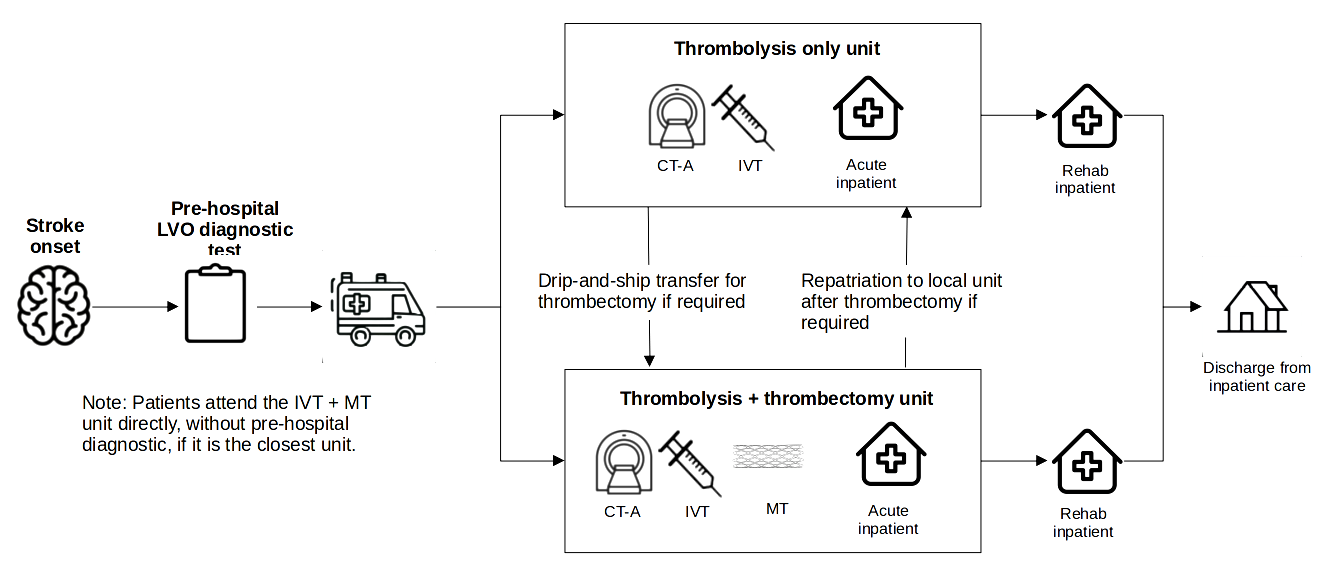
\includegraphics[width=1.0\textwidth]{./images/pathway}
\caption{Summary of patient flow through the emergency and in-patient rehabilitation stroke pathway. Abbreviations used are: LVO = Large Vessel Occlusions (a blockage of a large artery that may be suitable for thrombectomy); IVT = Intravenous Thrombolysis; MT = Mechanical thrombectomy; CT-A = CT-Angiogram (brain scan to confirm the type and location of the stroke).}
\label{fig:flow}
\end{figure}

Our research team uses various modelling techniques, including \textit{explainable machine learning} to identify the variation that occurs across different hospitals during the first few hours of stroke care. We use these models to understand the the source and impact of that variation on patients \cite{allen_using_2022, allen_use_2022}, identifying the variation that comes from hospitals and processes, rather than variation in local patient populations. We are working with the Sentinel Stroke National Audit Programme and NHS-England on reducing between hospital-variation in emergency stroke care. In this project we will build on previous and existing work, bringing it together into a single analysis framework, and extending work to cover looking at variation in inpatient lengths of stay, and an explainable machine learning analysis in variation in selection of patients for thrombectomy.

\subsubsection{Relevant prior and current work}

\begin{itemize}
    \item \textbf{Geographical analysis} - analysis of variation in access to thrombolysis and thrombectomy \cite{allen_maximising_2019}

    \item \textbf{Thrombolysis pathway and variation in patient selection} - analysis of between-hospital variation in the thrombolysis pathway using clinical pathway simulation and explainable machine learning \cite{allen_use_2022, pearn_what_2023}. Current work, as part of the NIHR SAMueL-2 project \footnote{\url{https://fundingawards.nihr.ac.uk/award/NIHR134326}} is focussing on an analysis of how between-hospital variation in selection of patients for thrombolysis effects patient outcomes. This work has produced a web tool \footnote{\url{https://stroke-predictions.streamlit.app/}}, including a health economics model, that is going in to use with the national stroke audit and NHS-England to help facilitate improvement in thrombolysis use, by working with lower thrombolysing units.

    \item \textbf{Pre-hospital pathway} - As part of the NIHR OptImIST programme \footnote{\url{https://fundingawards.nihr.ac.uk/award/NIHR202361}}, we are modelling the effect of pre-hopsital selection of patients for thrombectomy, the effect this is likely to have on time to thrombolysis and thrombectomy, and their outcomes (using a mathematical outcome model based on time to treatment).
    
\end{itemize}

\subsubsection{Proposed work}

See \textit{research questions and aims} below for more details. 

\begin{itemize}
    \item Analysis of variation in patient selection for thrombectomy

    \item Analysis of how variation in use of thrombolysis and thrombectomy effects in-patient length of stay

    \item Causal inference studies

    \item Production of a combined analytical pathway and web tool
    
\end{itemize}

\subsection{Why is this work important?}

Reperfusion treatment is the only emergency treatment for stroke proven to reduce disability. Unwanted variation in reperfusion treatment leads to avoidable variation in disability outcomes in stroke, which also has potential to cause unnecessary variation in downstream healthcare resource use. These methods are also potentially valuable in other healthcare settings where it is suspected that variation in healthcare and outcomes is due to variation in treatment processes and decisions rather than in differences in local patient populations.

\subsection{Review of existing evidence}

Studies have shown that reasons for low and varying thrombolysis rates are multi-factorial. Reasons include late presentation \cite{aguiar_de_sousa_access_2019}, lack of expertise \cite{aguiar_de_sousa_access_2019} or lack of clear protocols or training \cite{carter-jones_stroke_2011}, delayed access to specialists \cite{kamal_delays_2017}, and poor triage by ambulance or emergency department staff \cite{carter-jones_stroke_2011}. For many factors, the establishment of primary stroke centres has been suggested to improve the emergency care of patients with stroke and reduce barriers to thrombolysis \cite{carter-jones_stroke_2011}, with a centralised model of primary stroke centres leading to increased likelihood of thrombolysis \cite{lahr_proportion_2012, morris_impact_2014, hunter_impact_2013}. 

In addition to organisational factors, clinicians can have varying attitudes to which patients are suitable candidates for thrombolysis. In a discrete choice experiment \cite{de_brun_factors_2018}, 138 clinicians considered hypothetical patient vignettes, and responded as to whether they would give the patients thrombolysis. The authors concluded that there was considerable heterogeneity among respondents in their thrombolysis decision-making. Areas of difference were around whether to give thrombolysis to mild strokes, to older patients beyond 3 hours from stroke onset, and when there was pre-existing disability.

Based on national audit data from three years of emergency stroke admissions, we have previously built models of the emergency stroke pathway using clinical pathway simulation to examine the potential scale of the effect of changing two aspects of the stroke pathway performance (1. the in-hospital process speeds, and 2. the proportion of patients with a determined stroke onset time), and using machine learning to examine the effect of replicating clinical decision-making around thrombolysis from higher thrombolysing hospitals to lower thrombolysing hospitals \cite{allen_using_2022, allen_use_2022}. The machine learning model, which has 85\% accuracy (ROC-AUC = 0.92), learned whether any particular patient would receive thrombolysis in any particular emergency stroke centre. Using these models we found that it would be credible to target an increase in average thrombolysis in England and Wales, from 11\% to 18\%, but that each hospital should have its own target, reflecting differences in local populations. We found that the largest increase in thrombolysis use would come from replicating thrombolysis decision-making practice from higher to lower thrombolysing hospitals. Two other important factors influencing thrombolysis rates were determination of stroke onset time in some hospitals, and improving the speed of the in-hospital thrombolysis pathway.

We have extended the model to including explainability \cite{pearn_what_2023}. This revealed that lower thrombolysing hospitals, compared with higher thrombolysing hospitals, were particularly less likely to give thrombolysis to patients with 1) mild stroke, 2) imprecisely known onset time, 3) patient with prior disability, 4) any combination of those. This work is now forming the basis of a web tool \footnote{\url{https://stroke-predictions.streamlit.app/}} that allows stroke teams to compare their thrombolysis decisions to others, and to see how changing the pathway process can change the use and speed of thrombolysis, and the effect on patient outcomes.

We now wish to extend this work to include use of thrombectomy (including looking at any regional variation in patient selection), and the pre-hospital pathway. The latter also builds on our previous work looking at how to maximise access to thrombolysis and thrombectomy \cite{allen_maximising_2019}. Additionally we will use strengthen causal inference methodologies to test assumptions on how changing the pathway and patient selection will change patient outcomes.

\subsection{Research questions and aims}

\begin{itemize}
    \item \textbf{Analysis of variation in patient selection for thrombectomy} - how do thrombectomy centres vary in their selection of patients for thrombectomy, and what is the likely effect on outcomes from this variation?

    \item \textbf{Analysis of how variation in use of thrombolysis and thrombectomy effects in-patient length of stay} - how do thrombolysis and thrombectomy affect length of stay in acute and rehabilitation units?

    \item \textbf{Causal inference studies} - are observations from predictive models supported by causal inference studies, testing that any predictions made can be attributed to the assumed cause?

    \item \textbf{Production of a combined analytical pathway and web tool} - this tool with provide a national and regional analysis of current thrombolysis and thrombectomy use and provision, and enable an analysis of what an optimal system may look like, and the effect that would have on patients and health services. The tool will be developed and refined with co-production workshops, as we work with stroke teams on local thrombolysis and thrombectomy improvement. The web tool will combine:
    
    \begin{enumerate}
        \item Geographical analysis access to thrombolysis and thrombectomy. The map will identify which destination hospital would provide most likely best outcomes depending on type of stroke (of if stroke type is unknown)

        \item Clinical pathway simulation (including the pre-hospital pathway) - showing how optimisation of the pathway may effect thrombolysis and thrombectomy use and speed.

        \item Explainable machine-learning analysis of variation in choice of patients for thrombolysis and thrombectomy (with causal inference methodology to give further confidence in modelling).

        \item A health economics model based on patient outcomes, extending patient outcome results to expected QALY (quality-adjusted life years).
    \end{enumerate} 
    
\end{itemize}

\subsection{Project Plan}

\subsubsection{Data}

We use anonymous patient-level data from the Sentinel Stroke National Audit Programme (SSNAP, \url{https://www.strokeaudit.org/}. SSNAP collects data on essentially all emergency stroke units, from all stroke units in England, Wales, and Northern Ireland. The data includes a wide range of information such as data on times throughout the stroke pathway from stroke onset, pre-stroke disability (modified Rankin Scale, mRS), a breakdown of stroke symptoms using the NIHSS stroke scale, reperfusion treatment given (and timing), comorbidities, death in hospital, disability at discharge from inpatient care, and 6 month follow-up disability (the latter is complete for about 35\% of discharged patients). Data is collected for about 85,000 patients each year, 10-11\% of whom receive thrombolysis, and about 3\% now receiving thrombectomy.


